% 设定文章类型与编码格式
\documentclass[UTF8]{article}	
\usepackage[UTF8]{ctex}     % 设置文档为中文语言

% 图片设置
\usepackage{graphicx}  % 支持 jpg, png, eps, pdf 图片 
\usepackage{float}     % 图表位置浮动设置 (H) Here, (H!) Here forced
\usepackage{subcaption} % 用于子图和小图注 

% 文章页面margin设置
\usepackage[a4paper]{geometry}
\geometry{top=0.6in}
\geometry{bottom=0.4in}
\geometry{left=0.5in}
\geometry{right=0.5in}   % 设置上下左右页边距
\geometry{marginparwidth=1.5cm}    % 设置边注距离(注释、标记等)

% 页眉页脚设置
\usepackage{fancyhdr}   %宏包:页眉页脚设置
    \pagestyle{fancy}
    \fancyhf{}
    %\cfoot{\thepage}   % 页码
    \renewcommand\headrulewidth{1pt}
    \renewcommand\footrulewidth{0pt} 
    \usepackage{fontawesome}    % 宏包:更多符号与图+** (用于插入 GitHub 图标等)
    \lhead{\footnotesize
    \href{https://github.com/YiDingg/UCAS-BasicPhysicsExperiment}{\color{black}\faGithub\ https://github.com/YiDingg/UCAS-BasicPhysicsExperiment}}
    \rhead{\small 实验专用作图纸}
    %\lhead{\footnotesize\href{https://github.com/YiDingg/LatexNotes}{\color{black}\faGithub\ https://github.com/YiDingg/LatexNotes}}


% 文章默认字体设置
\usepackage{fontspec}   % 宏包:字体设置
\setmainfont{SimSun}    % 设置中文字体为宋体字体
\setCJKmainfont[AutoFakeBold=3]{SimSun} % 设置加粗字体为 SimSun 族,AutoFakeBold 可以调整字体粗细
\setmainfont{Times New Roman} % 设置英文字体为Times New Roman

\usepackage{hyperref}  % 宏包:生成超链接
\hypersetup{
        colorlinks=true,    % false:边框链接 ; true:彩色链接
        citecolor={blue},    % 文献引用颜色
        linkcolor={blue},   % 目录 (我们在目录处单独设置),公式,图表,脚注等内部链接颜色
        urlcolor={orange},    % 网页 URL 链接颜色,包括 \href 中的 text
        % cyan 浅蓝色 
        % magenta 洋红色
        % yellow 黄色
        % black 黑色
        % white 白色
        % red 红色
        % green 绿色
        % blue 蓝色
        % gray 灰色
        % darkgray 深灰色
        % lightgray 浅灰色
        % brown 棕色
        % lime 石灰色
        % olive 橄榄色
        % orange 橙色
        % pink 粉红色
        % purple 紫色
        % teal 蓝绿色
        % violet 紫罗兰色
    }

% 外源代码插入设置
    % matlab 代码插入设置
    \usepackage{matlab-prettifier}
        \lstset{style=Matlab-editor}    % 继承 matlab 代码高亮 , 此行不能删去
    \usepackage[most]{tcolorbox} % 引入tcolorbox包 
    \usepackage{listings} % 引入listings包
        \tcbuselibrary{listings, skins, breakable}
        \newfontfamily\codefont{Consolas} % 定义需要的 codefont 字体
        \lstdefinestyle{MatlabStyle_inc}{   % 插入代码的样式
            language=Matlab,
            basicstyle=\footnotesize\ttfamily\codefont,    % ttfamily 确保等宽 
            breakatwhitespace=false,
            breaklines=true,
            captionpos=b,
            keepspaces=true,
            numbers=left,
            numbersep=15pt,
            showspaces=false,
            showstringspaces=false,
            showtabs=false,
            tabsize=2,
            xleftmargin=15pt,   % 左边距
            %frame=single, % single 为包围式单线框
            frame=shadowbox,    % shadowbox 为带阴影包围式单线框效果
            %escapeinside=``,   % 允许在代码块中使用 LaTeX 命令 (此行无用)
            %frameround=tttt,    % tttt 表示四个角都是圆角
            framextopmargin=0pt,    % 边框上边距
            framexbottommargin=0pt, % 边框下边距
            framexleftmargin=5pt,   % 边框左边距
            framexrightmargin=5pt,  % 边框右边距
            rulesepcolor=\color{red!20!green!20!blue!20}, % 阴影框颜色设置
            %backgroundcolor=\color{blue!10}, % 背景颜色
        }
        \lstdefinestyle{MatlabStyle_src}{   % 插入代码的样式
            language=Matlab,
            basicstyle=\small\ttfamily\codefont,    % ttfamily 确保等宽 
            breakatwhitespace=false,
            breaklines=true,
            captionpos=b,
            keepspaces=true,
            numbers=left,
            numbersep=15pt,
            showspaces=false,
            showstringspaces=false,
            showtabs=false,
            tabsize=2,
        }
        \newtcblisting{matlablisting}{
            %arc=2pt,        % 圆角半径
            % 调整代码在 listing 中的位置以和引入文件时的格式相同
            top=0pt,
            bottom=0pt,
            left=-5pt,
            right=-5pt,
            listing only,   % 此句不能删去
            listing style=MatlabStyle_src,
            breakable,
            colback=white,   % 选一个合适的颜色
            colframe=black!0,   % 感叹号后跟不透明度 (为 0 时完全透明)
        }
        \lstset{
            style=MatlabStyle_inc,
        }

\begin{document}

% 50 x 50 
\section*{实验作图专用纸 (50 $\times$ 50)}

\begin{figure}[H]\centering
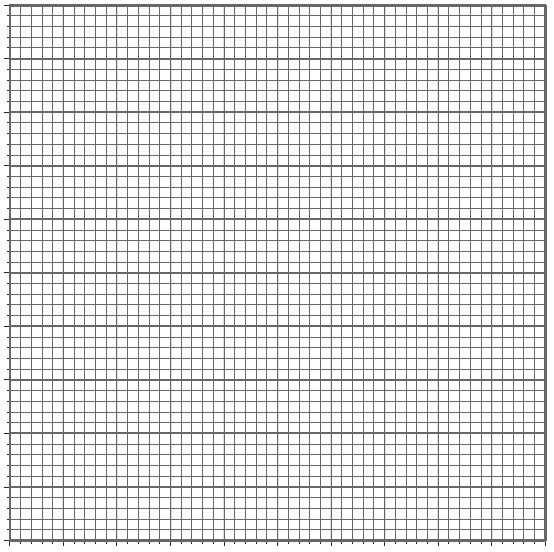
\includegraphics[width=\columnwidth]{assets/50x50.pdf}
\end{figure}

\begin{figure}[H]\centering
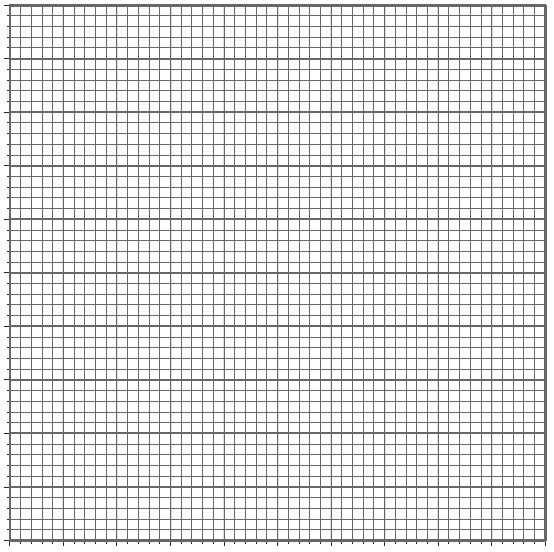
\includegraphics[width=0.8\columnwidth]{assets/50x50.pdf}
\end{figure}

\begin{figure}[H]\centering
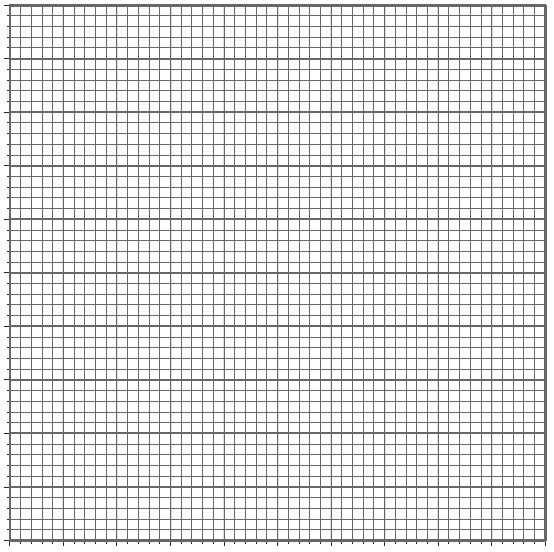
\includegraphics[width=0.65\columnwidth]{assets/50x50.pdf}
\end{figure}

\begin{figure}[H]\centering
\begin{subfigure}[b]{0.46\columnwidth}\centering
    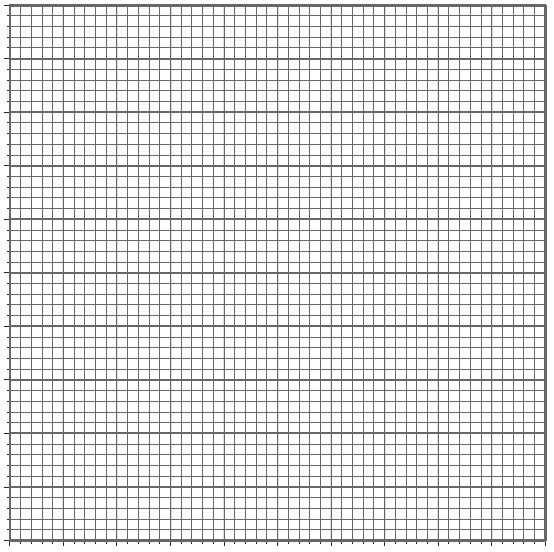
\includegraphics[width=\columnwidth]{assets/50x50.pdf}
\end{subfigure}\hfill
\begin{subfigure}[b]{0.46\columnwidth}\centering
    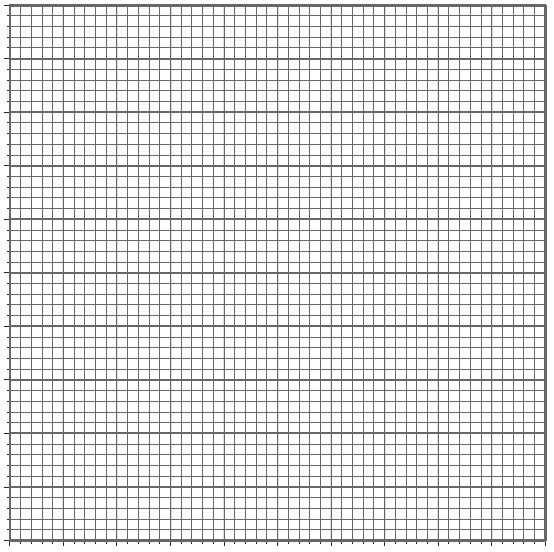
\includegraphics[width=\columnwidth]{assets/50x50.pdf}
\end{subfigure}
\end{figure}

\begin{figure}[H]\centering
\begin{subfigure}[b]{0.46\columnwidth}\centering
    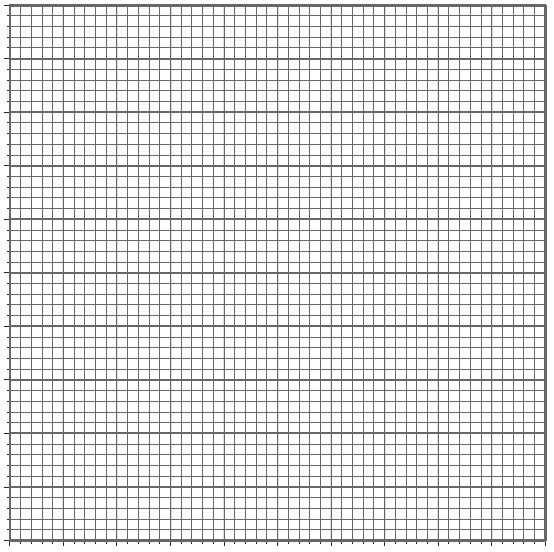
\includegraphics[width=\columnwidth]{assets/50x50.pdf}
\end{subfigure}\hfill
\begin{subfigure}[b]{0.46\columnwidth}\centering
    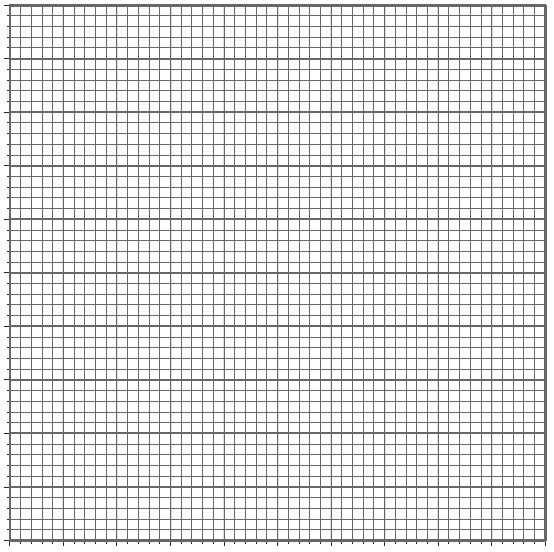
\includegraphics[width=\columnwidth]{assets/50x50.pdf}
\end{subfigure}
\end{figure}
\begin{figure}[H]\centering
    \begin{subfigure}[b]{0.46\columnwidth}\centering
        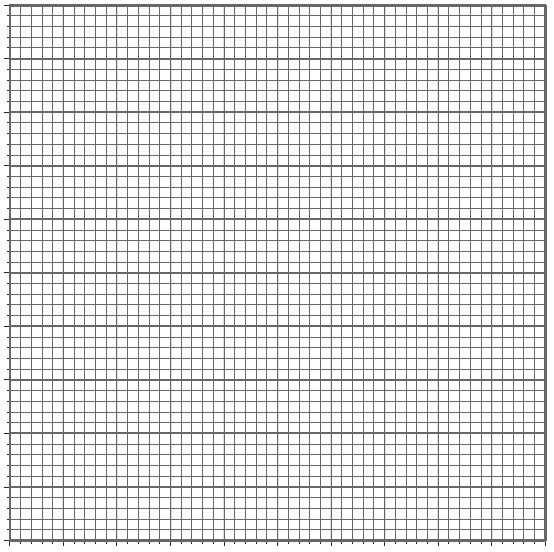
\includegraphics[width=\columnwidth]{assets/50x50.pdf}
    \end{subfigure}\hfill
    \begin{subfigure}[b]{0.46\columnwidth}\centering
        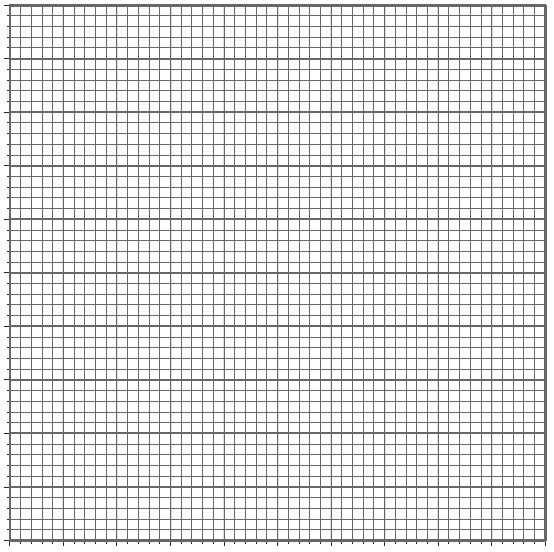
\includegraphics[width=\columnwidth]{assets/50x50.pdf}
\end{subfigure}
\end{figure}
\begin{figure}[H]\centering
    \begin{subfigure}[b]{0.46\columnwidth}\centering
        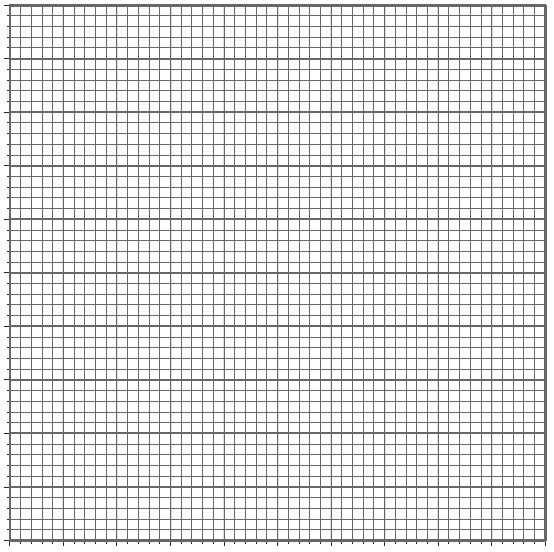
\includegraphics[width=\columnwidth]{assets/50x50.pdf}
    \end{subfigure}\hfill
    \begin{subfigure}[b]{0.46\columnwidth}\centering
        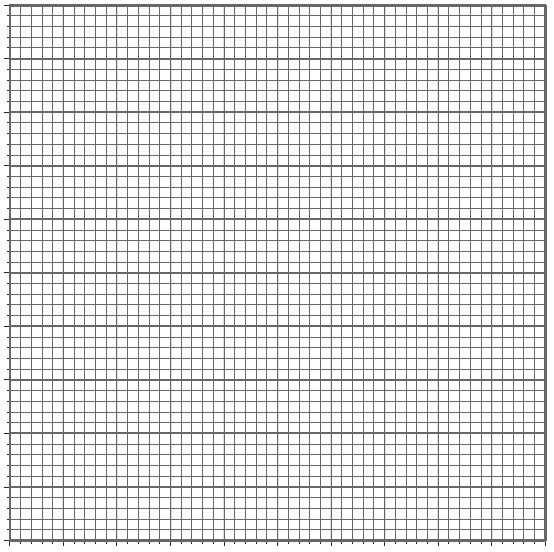
\includegraphics[width=\columnwidth]{assets/50x50.pdf}
    \end{subfigure}
\end{figure}




% 100 x 50 

\newpage
\section*{实验作图专用纸 (100 $\times$ 50)}

\begin{figure}[H]\centering
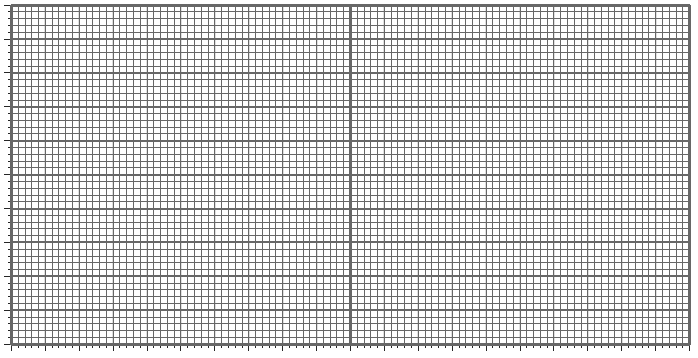
\includegraphics[width=\columnwidth]{assets/100x50.pdf}
\end{figure}
\begin{figure}[H]\centering
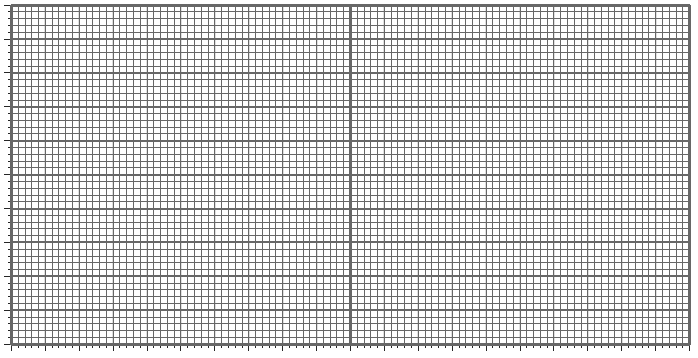
\includegraphics[width=\columnwidth]{assets/100x50.pdf}
\end{figure}

\begin{figure}[H]\centering
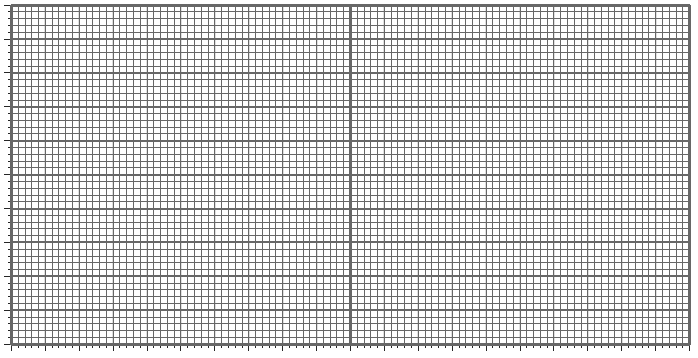
\includegraphics[width=0.8\columnwidth]{assets/100x50.pdf}
\end{figure}

\begin{figure}[H]\centering
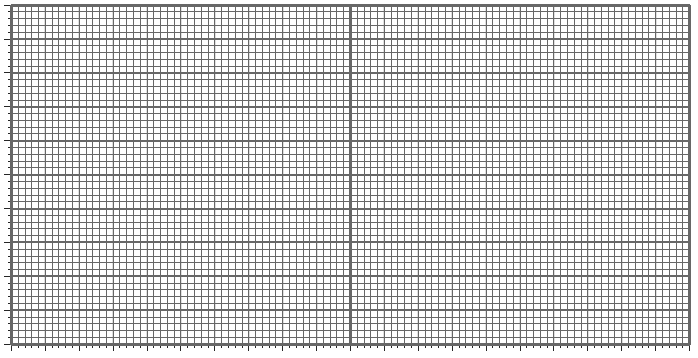
\includegraphics[width=0.65\columnwidth]{assets/100x50.pdf}
\end{figure}

\begin{figure}[H]\centering
\begin{subfigure}[b]{0.5\columnwidth}\centering
    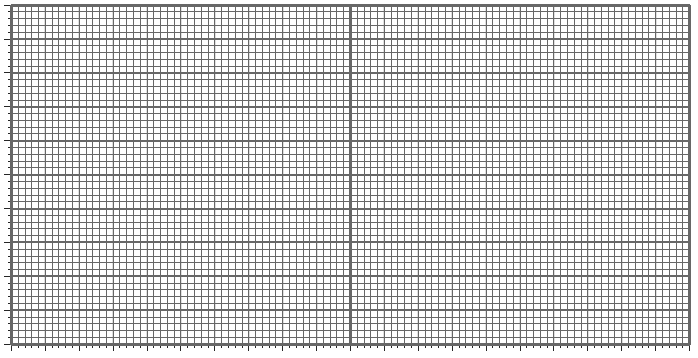
\includegraphics[width=\columnwidth]{assets/100x50.pdf}
\end{subfigure}\hfill
\begin{subfigure}[b]{0.5\columnwidth}\centering
    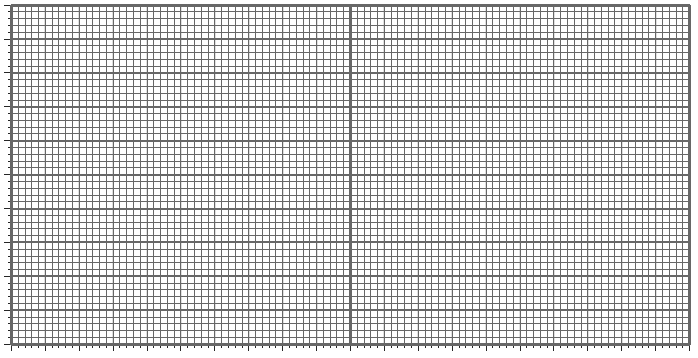
\includegraphics[width=\columnwidth]{assets/100x50.pdf}
\end{subfigure}
\end{figure}

\begin{figure}[H]\centering
\begin{subfigure}[b]{0.5\columnwidth}\centering
    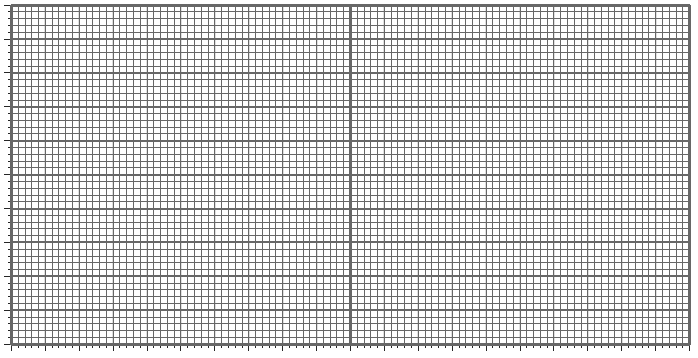
\includegraphics[width=\columnwidth]{assets/100x50.pdf}
\end{subfigure}\hfill
\begin{subfigure}[b]{0.5\columnwidth}\centering
    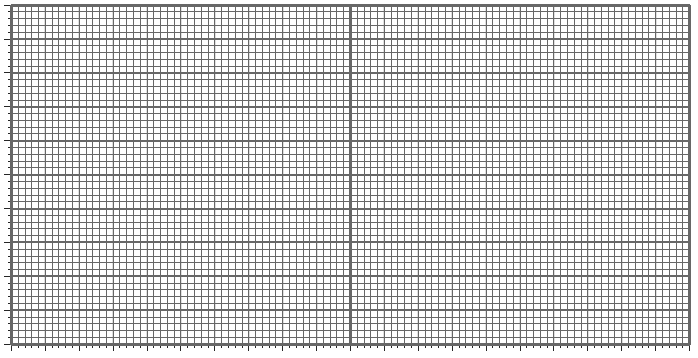
\includegraphics[width=\columnwidth]{assets/100x50.pdf}
\end{subfigure}
\end{figure}


% 100 x 100
\newpage
\section*{实验作图专用纸 (100 $\times$ 100)}

\begin{figure}[H]\centering
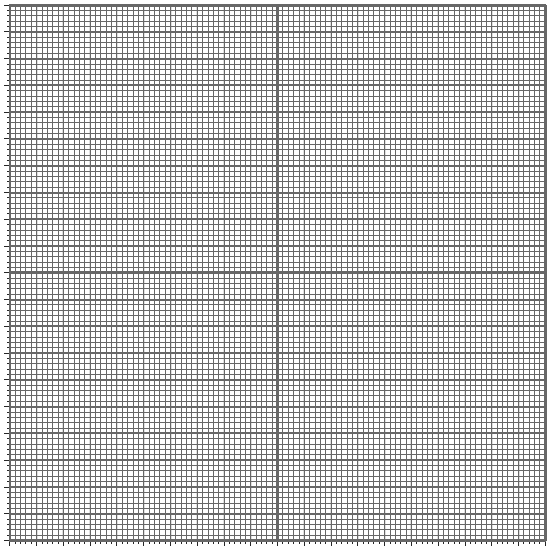
\includegraphics[width=\columnwidth]{assets/100x100.pdf}
\end{figure}

\begin{figure}[H]\centering
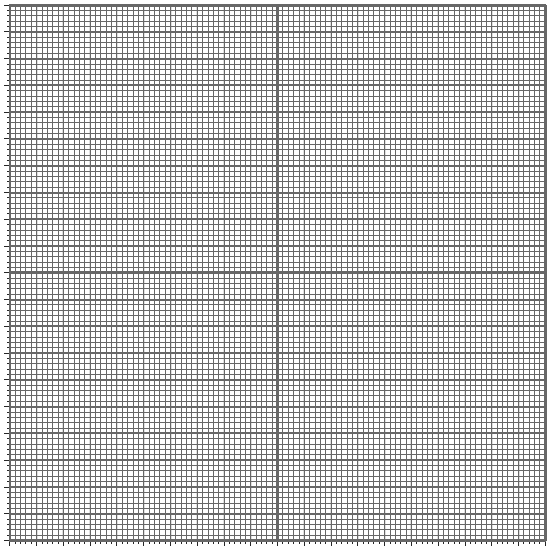
\includegraphics[width=0.8\columnwidth]{assets/100x100.pdf}
\end{figure}

\begin{figure}[H]\centering
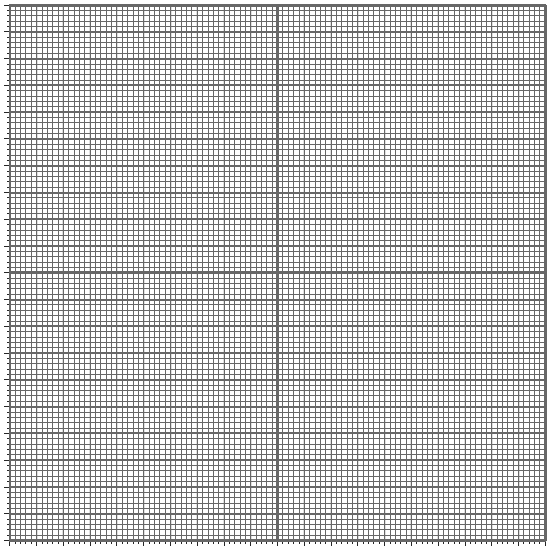
\includegraphics[width=0.65\columnwidth]{assets/100x100.pdf}
\end{figure}

\begin{figure}[H]\centering
\begin{subfigure}[b]{0.5\columnwidth}\centering
    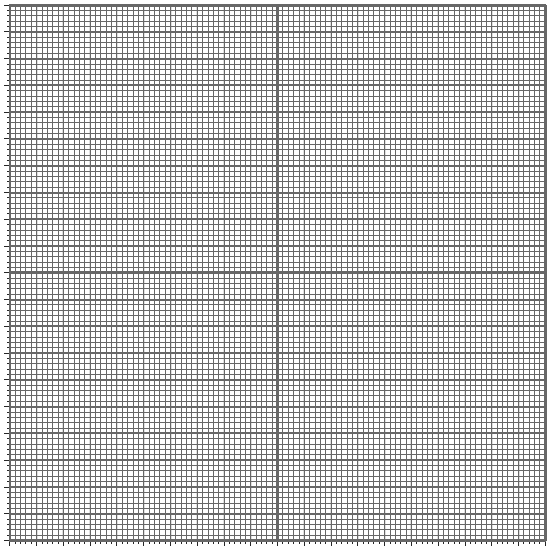
\includegraphics[width=\columnwidth]{assets/100x100.pdf}
\end{subfigure}\hfill
\begin{subfigure}[b]{0.5\columnwidth}\centering
    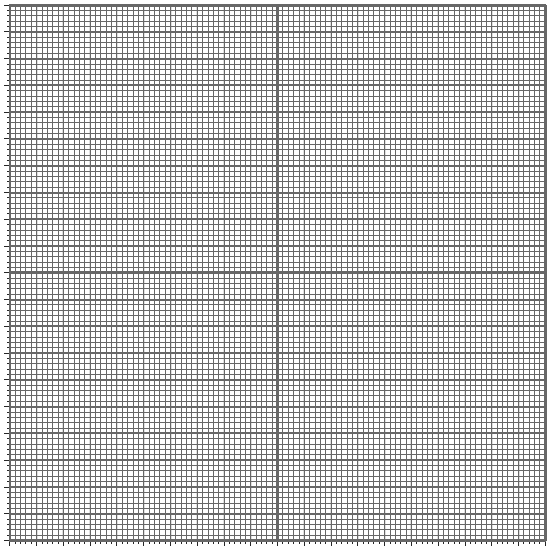
\includegraphics[width=\columnwidth]{assets/100x100.pdf}
\end{subfigure}
\end{figure}

\begin{figure}[H]\centering
\begin{subfigure}[b]{0.5\columnwidth}\centering
    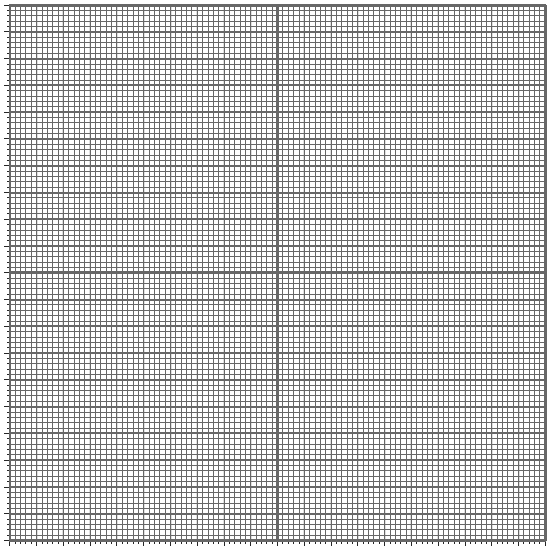
\includegraphics[width=\columnwidth]{assets/100x100.pdf}
\end{subfigure}\hfill
\begin{subfigure}[b]{0.5\columnwidth}\centering
    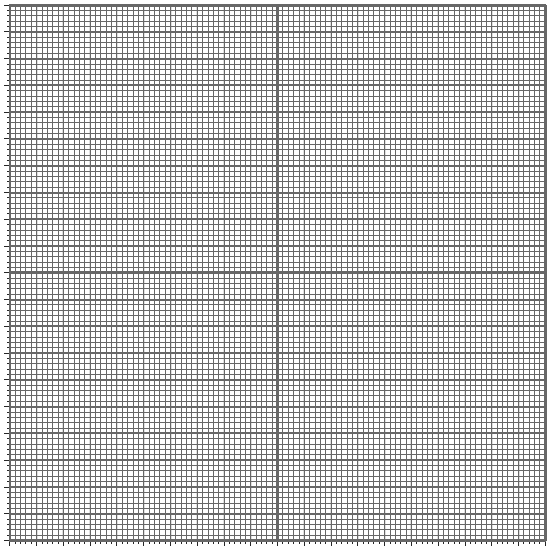
\includegraphics[width=\columnwidth]{assets/100x100.pdf}
\end{subfigure}
\end{figure}

\begin{figure}[H]\centering
    \begin{subfigure}[b]{0.5\columnwidth}\centering
        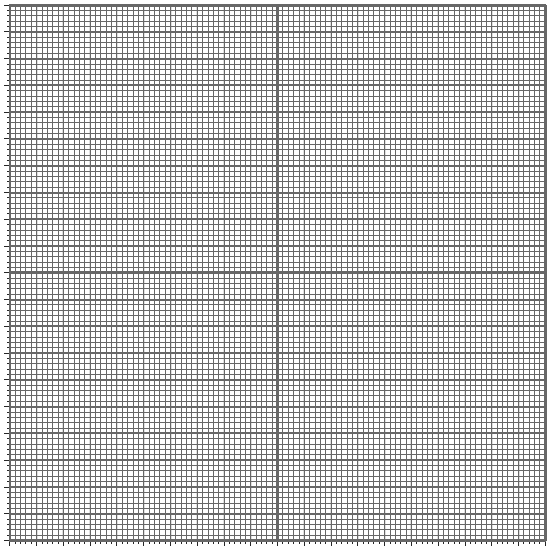
\includegraphics[width=\columnwidth]{assets/100x100.pdf}
    \end{subfigure}\hfill
    \begin{subfigure}[b]{0.5\columnwidth}\centering
        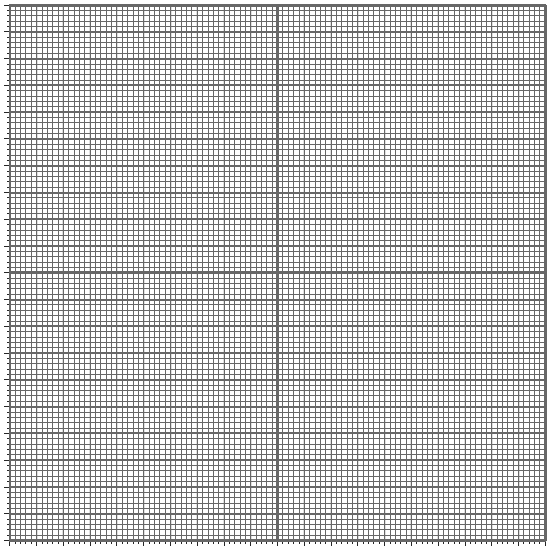
\includegraphics[width=\columnwidth]{assets/100x100.pdf}
    \end{subfigure}
\end{figure}


\newpage
\section*{附录 \hspace*{10pt} Matlab 源码}
\lstinputlisting{d:/a_RemoteRepo/GH.MatlabCodes/本科课程代码/基础物理实验/PlotPaper_mflie.m}

\end{document}